% !TeX spellcheck = en_GB
\documentclass[12pt,a4paper,twoside]{article}
\usepackage[english]{babel}
\usepackage{amsmath}
\usepackage{amsthm}
\usepackage{amssymb}
\usepackage{amsfonts}
\usepackage{graphicx}
\usepackage{mathtools}
\usepackage[utf8]{inputenc}
\usepackage{csquotes}
\usepackage[hidelinks, final]{hyperref}
\usepackage[printonlyused]{acronym}
\usepackage{color}
\usepackage[svgnames]{xcolor}
\usepackage{transparent}
%the following is for R-code
\usepackage{xspace}
\usepackage{url}
\usepackage{listings}

\lstset{
	basicstyle=\small\ttfamily,
	stringstyle=\color{DarkGreen},
	otherkeywords={0,1,2,3,4,5,6,7,8,9},
	morekeywords={TRUE,FALSE},
	deletekeywords={data,frame,length,as,character},
	keywordstyle=\color{blue},
	commentstyle=\color{DarkGreen},
}
\lstnewenvironment{rc}[1][]{\lstset{language=R}}{}
\newcommand{\ri}[1]{\lstinline{#1}}  %% Short for 'R inline'

\lstset{language=R}             % Set R to default language

\graphicspath{{img/}}
\usepackage[%
backend=biber,
url=false,
style=numeric,
sorting=none,
maxnames=4,
minnames=3,
maxbibnames=99,
giveninits,
uniquename=init]{biblatex}
\addbibresource{bachelor_thesis_julien_caselmann.bib}
%TODO last: many weird sources, fix them
%TODO last: R skripte, die plots generiert haben in einen anhang
%TODO last: sort sources numerically in every multi-cite bracket

%TODO: disclaimer am anfang: anti-vax, anti-vaxxer,anti-immu,anti-vaccination will be used austauschingly as per general convention

\newtheorem{definition}{Definition}[section]
\newtheorem{thm}{Theorem}[section]
\newtheorem{lem}{Lemma}[section]
\newtheorem{prop}{Proposition}[section]
\newtheorem{claim}{Claim}[section]
\newtheorem{model}{Model}[section]

\setlength{\voffset}{-28.4mm}
\setlength{\hoffset}{-1in}
\setlength{\topmargin}{20mm}
\setlength{\oddsidemargin}{25mm}
\setlength{\evensidemargin}{25mm}
\setlength{\textwidth}{160mm}

\setlength{\parindent}{0pt}

\setlength{\textheight}{235mm}
\setlength{\footskip}{20mm}
\setlength{\headsep}{50pt}
\setlength{\headheight}{0pt}


\begin{document}
\pagestyle{empty}
%%%% Title page
\begin{titlepage}
\begin{center}

\includegraphics{img/TUMlblack.png}\\[3mm]
\sf
{\Large
  Technische Universit\"at M\"unchen\\[5mm]
  Department of Mathematics\\[8mm]
}
\normalsize

\includegraphics{img/TUMlMblack.png}\\[15mm]

Bachelor's Thesis\\[15mm]

{\Huge
  The Dynamics of Vaccination Hesitancy
}
\bigskip

\normalsize

Julien Caselmann
\end{center}
\vspace*{75mm}

Supervisor: Prof. Dr. Johannes M\"uller
\medskip

Advisor: Prof. Dr. Johannes M\"uller
\medskip

Submission Date: 01.07.2020

\end{titlepage}
%%%% The following has to be signed by hand!

\vspace*{150mm}

I assure the single handed composition of this bachelor's thesis only supported by declared resources.
\bigskip

Munich, \today \newline

\begin{figure}[h!]
	\hfill
	\begin{minipage}{.4\textwidth}\centering
		\def\svgwidth{350pt}
		\input{img/unterschrift_julien_caselmann.pdf_tex}
	\end{minipage}	
\end{figure}


\newpage
%%%% Summary in german
\section*{Zusammenfassung}
Trotz nachweislichen/nachgewiesenen? Zusammenhängen zwischen niedriger Impfrate und dem Wiederauftauchen bereits ausgerotteter Krankheiten, sind die durchschnittlichen Impfzahlen in Deutschland bei Weitem nicht hoch genug, um Herdenimmunität zu gewährleisten. Das Ziel der Bachelorarbeit ist es, dieses paradoxale Impfverhalten und die zugrundeliegenden Dynamiken durch Kombinierung zweier bekannter Modelle und Einbeziehung von Prozessen der Meinungsbildung zu verstehen und zu analysieren. Zunächst werden bekannte Ansätze zur Modellierung von Impfskepsis, sowie Meinungsbildung mit und ohne Rücksicht auf Filterblasen präsentiert. Anschließend wird ein kombiniertes Modell, bestehend aus den Ansätzen von Bauch \cite{Bauch2012}, Müller und Tellier \textbf{cite} und dem Konzept von Pay-off Funktionen aus der Wirtschaftsmathematik, aufgestellt und eine Bifurkationsanalyse durchgeführt. Es treten Pitchfork-, sowie Sattel-Knoten-Bifurkationen für einen Spezialfall und eine allgemeine Hopf-Bifurkation auf. Eine Takens-Bogdanov-Bifurkation wird vermutet, in dieser Arbeit aber nicht nachgewiesen. Im letzten Abschnitt wird das Modell auf Impfdaten des \acfp{RKI}, die die bundesweite Impfabdeckung gegen C-Meningokokken auf Kreisebene darstellen, gefittet. Das Modell fittet gut/schlecht, mal schauen.

\section*{Abstract}
%TODO: muss dat?
Have todo?
\newpage
\tableofcontents
\newpage

%%%% Page numbering restarts here
\pagenumbering{arabic}
\pagestyle{headings}

\newpage

%if you do not use this, delete following packages in preamble:
%acronym

\section*{Abbreviations}

\begin{acronym}[STIKO]%write longest acronym here for nice formatting purposes
	%to use them write \ac{KPMG} or \acp{KPMG for plural in the text}
	\acro{RKI}{Robert-Koch-Institut}
	\acroplural{RKI}[RKI]{Robert-Koch-Instituts}
	\acro{SIR}{Susceptible, Infected, Recovered}
	\acro{BCM}{bounded-confidence model}
	\acro{WHO}{World Health Organization}
	\acro{BVM}{biased voter model}
	\acro{AfD}{Alternative für Deutschland}
	\acro{GDR}{German Democratic Republic}
	\acro{ODE}{Ordinary Differential Equation}
	\acro{STIKO}{Ständige Impfkommission}
	\acro{HIV}{Human Immunodeficiency Viruses}
	\acro{MMR}{Measles-Mumps-Rubella}
	%if one acronym's plural form is more than just an "s" attached, you have to specify that:
	\acro{SQ}{sexy query}
	\acroplural{SQ}[SQs]{sexy queries}
\end{acronym}

\newpage

\listoffigures

\newpage

\section{Introduction}

The personal pursuit of health, wealth and happiness should be a familiar concept to anyone. Everybody wishes to do the best they can to be the happiest they can, the longest they can. Governmental institutions involved with Public Health also strive for health, but on a larger scale. They aim at the best possible health conditions for the largest possible number of individuals at the same time. Interestingly, the interests and opinions of citizens and Public Health institutions do not always coincide, especially not when it comes to vaccination. As the British philosopher Jeremy Bentham saw society in the second half of the 18$^{\textnormal{th}}$ century, the human was nothing more than a benefit-maximizer, that pursued his personal interests without any respect of his environment \cite{Bentham1988}. So he introduced the greatest happiness principle, a concept based on the opinion that an action was considered as good if it was beneficial for the most possible individuals, and considered as bad, if it harmed the community. More or less parallel to this principle, modern medicine and research have shown the effect of herd-immunity, and how a disease can disappear within a population, if enough individuals are immunised against it \cite{Gordis2014}. Following these lines of thoughts, western governments and their Public Health institutions have shown a tendency in the past few years to impose or at least encourage vaccination \cite{KBV2019, Drew2019}. But this did not fit the personal needs every individual developed, valued and wanted to see pursued, so very soon, vaccine opponents appeared. One of the ``anti-vax pioneers" was Reverend Edmund Massey, who lived in the 18$^{\textnormal{th}}$ century and described vaccination as a ``diabolical operation" \cite{MASSEY2018}. The opposition to vaccination has always been present since then and has grown remarkably in the past, mostly after being empowered by studies that published allegedly shocking correlations between immunisation shots and the emergence of severe disease or disabilities \cite{Rao2011}. A well-known example would be the study from Wakefield et al. in 1998 that pretended to have revealed the \ac{MMR} vaccine was very likely to predispose to autism any child who had taken the shot \cite{Wakefield1998}. Despite the very small sample size $n = 12$, utterly speculative conclusions and even having been refuted by multiple studies such as \cite{DeStefano2013, Dales2001, Taylor1999}, those claims received an enormous amount of publicity and had a tremendous impact on the way people perceived vaccines \cite{Rao2011}.\newline

One tends to quickly classify and label individuals related to either the pro or anti-vax camp, but \textbf{Quelle finden} shows that vaccination opponents as well as proponents come from various social and educational backgrounds or cultures%TODO: quelle? didnt find one on the first try
. The main difference between those two camps seems to be the willingness to propagate their ideas amongst others. While individuals who do immunise themselves regularly are less involved in the propagation of vaccines than the government or health institutions, the so-called ``anti-vaxxers" are pretty active and way less peripheral when it comes to spread their opinion \cite{Johnson2020}. Additionally, the anti-vax movement is has been shown to be very influential and misleading during the opinion formation process, because of their excessive use of emotive and rhetorical appeals and their tendency to cite medical studies and draw wrong conclusions afterwards \cite{Davies2002}.\newline

Furthermore, religious communities with rather extreme opinions have shown to be a huge danger for the public health, as their general rejection of vaccines caused severe diseases to reappear amongst them and led to a large amount of casualties, like the multiple outbreaks of measles in communities of Christian Scientists \cite{Novotny1988}. In Nigeria, simple, non fact-based assumptions that the vaccine against poliovirus transmitted \ac{HIV} scattered all the immunisation efforts that had been made in the previous 15 years \cite{Pincock2004}. As presented by Hussain in \cite{Hussain2018}, this has not been the only case where rumours and fake news were an impactful factor for the decision finding in the population.\newline

Apart from religious or ideological filter bubbles, vaccines are far away from being generally accepted. The results of the survey requested by the European Commission concerning Europeans' attitudes towards vaccinations \cite{KantarBelgium2019}, represented in Figure \ref{fig:vaccine_mistrust_eu} below, show a non-negligible mistrust in vaccines amongst European citizens. Despite being such a minority, anti-vax groups show a remarkable impact on society and Hussain even calls it ``A regression in Modern Medicine" in \cite{Hussain2018}. This work will address this phenomenon and try to understand it, by first presenting various existing models that all have tackled the problem with different creative approaches and eventually proposing an own modelling idea with the aim of integrating an opinion forming process into a compartmental modelling approach.

\begin{figure}[h!]
	\centering %(or not)
	\caption{Reasons for not having any vaccination in the EU
		\label{fig:vaccine_mistrust_eu} \cite{KantarBelgium2019}}
	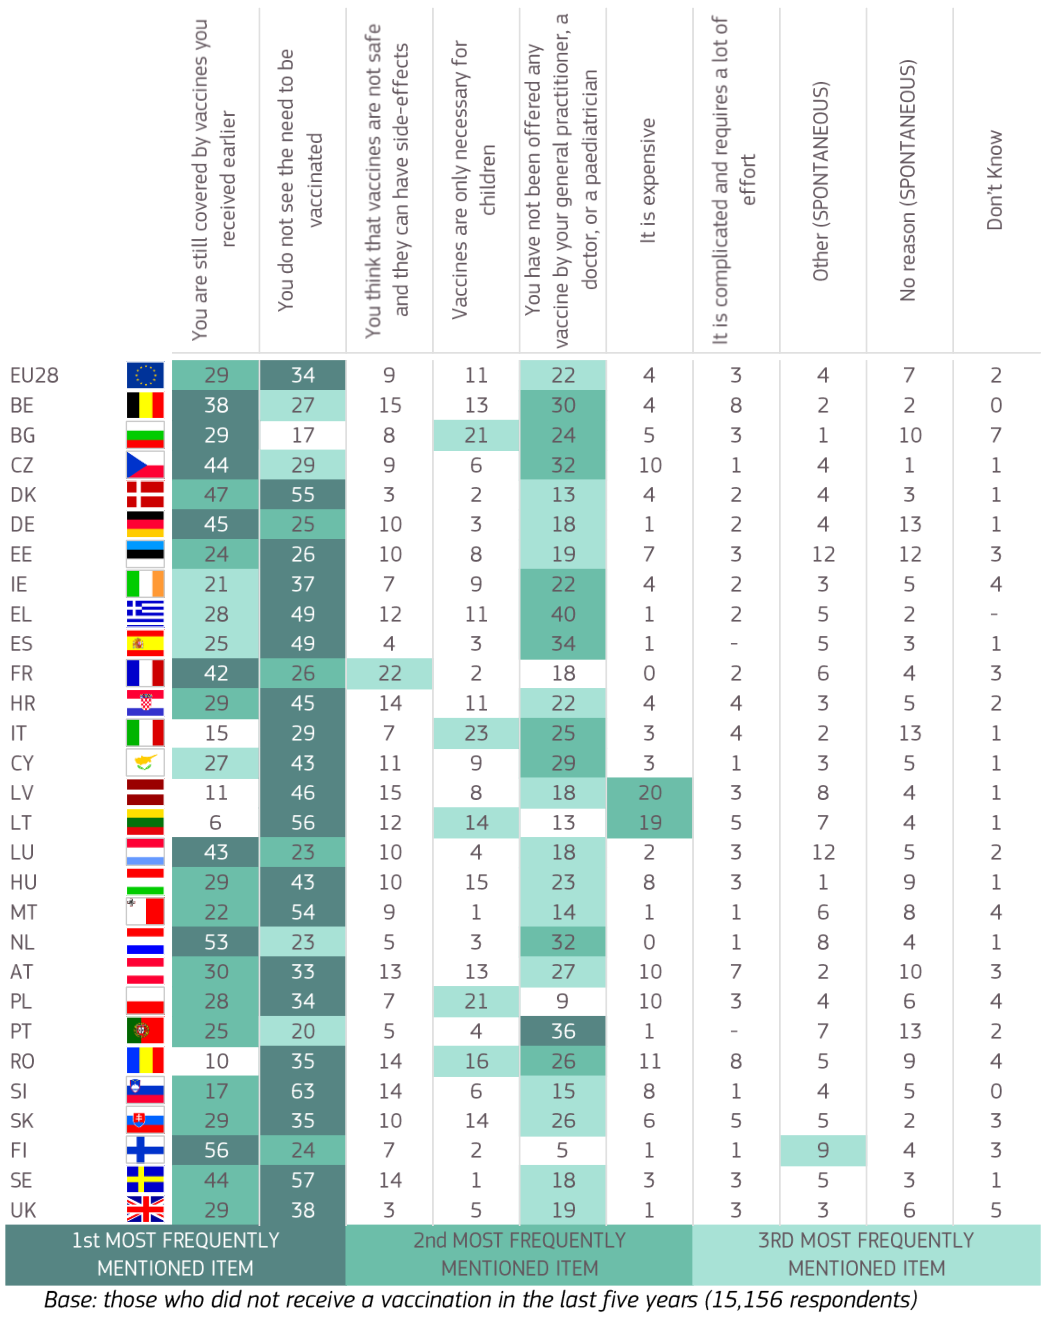
\includegraphics[scale=0.387]{img/vaccine_hesitancy_EU_MULTIPLE_ANSWERS.png}
\end{figure}

\newpage

\section{Hesitancy Model}
Firstly, we will have to take a look at a way to model vaccination hesitancy and try to understand, how the individuals with a pro-vaccination opinion behave and where the dependencies of their behaviour lie. The medical/biological approach over the past few years has inter alia been to compose literature reviews and to form working groups such as in \cite{MacDonald2015} to be able to define so-called ``vaccine hesitancy determinants". Those are categories of reasons, for which individuals would decide not to take a vaccine. Then, a mathematical model of the dynamics had to be found, which takes into account the found determinants and one can analyse mathematically to potentially define explicit influence factors for the vaccine hesitancy dynamics. 

Over time, several different models have been elaborated, but only one will be presented in this thesis: the significant work of Bauch and Bhattacharyya in \cite{Bauch2012}. They developed a behaviour-incidence model with the aim to describe the dynamics of the number of vaccinated subjects $x$ depending on different factors such as vaccine risk, efficacy and the number of infectious persons. To get a better overview, all of the variables used in the model will be listed here:
\begin{align}\label{table:bauch_model_variables}
\begin{split}
S &: \textnormal{number of susceptible subjects in the population}\\
I &: \textnormal{number of infected subjects in the population}\\
x &: \textnormal{relative number of vaccinated subjects in the population}\\
\mu &: \textnormal{birth and death rate of the population}\\
\epsilon &: \textnormal{vaccine efficacy}\\
\beta &: \textnormal{infection rate}\\
\tau &: \textnormal{case importation rate}\\
\gamma &: \textnormal{recovery rate}\\
\kappa &: \textnormal{scale factor}\\
\omega &: \textnormal{vaccine penalty}
\end{split}
\end{align}

The vaccine penalty $\omega$ basically describes the amount of risk a vaccination brings and $\kappa$ is a measure for the response speed of the population to external influences. A high value for $\kappa$ means that they change their opinion (pro-vaccine $\rightleftarrows$ contra-vaccine) immediately, a low $\kappa$ stands for a very slow reaction. The variables $S$ and $I$ follow the convention from the well-studied \ac{SIR} model developed by Kermack and McKendrick in 1927 (for more details, see \cite{Muller2015}). We may now define the model:
\begin{model}[\textbf{Behaviour-incidence model by \cite{Bauch2012}}]\label{model:bauch}
	Let the context be defined as in \eqref{table:bauch_model_variables}. Then, the dynamics of the according behaviour-incidence model are:
	\begin{align}
	\begin{split}
	\frac{dS}{dt} &= \mu\left(1-\epsilon x\right) - \mu S - \beta SI - \tau S\\
	&\\
	\frac{dI}{dt} &= -\mu I + \beta SI - \gamma I + \tau S\\
	&\\
	\frac{dx}{dt} &= \kappa x\left(1 - x\right)\left(I - \omega\right)
	\end{split}
	\end{align}
\end{model}

The modelling idea is that every person starts in the group of susceptible individuals $S$ and either stays in $S$, moves to the group of infected individuals $I$, or gets the vaccine and immediately jumps into the group of recovered subjects $R$. As the main interest of this model is the dynamics of vaccinated subjects $x$ and once an individual gets into $R$, a return to $S$ or $I$ is impossible, it is assumed that the recovered have left the model, thus are not considered in Model \ref{model:bauch}. The dynamics of $S$ are pretty straight-forward: the only way to get into $S$, is to get born into the population, so the only positive term is the birth rate $\mu$. On the other hand, there are multiple ways to get ot of $S$: an individual might either die $\left(-\mu S\right)$, get infected by one individual of $I$ $\left(-\beta SI\right)$, be born as a child of vaccinated subjects and get an immunisation shot at birth $\left(-\mu\epsilon x\right)$ or come from another population as an infected and immediately jump from $S$ to $I$ $\left(-\tau S\right)$.\newline

$I$ is designed in a similar way: newly infected subjects were either infected in the observed population $\left(+\beta SI\right)$ or came from another population and brought the disease with them $\left(+\tau S\right)$. Again, an individual leaves $I$ at death $\left(-\mu I\right)$ or after recovering from the disease $\left(-\gamma I\right)$.\newline

Finally, let us take a look at the dynamics of vaccinated subjects. Their growth factor consists of three parts: the response speed $\kappa$ as described above, the amount of anti-vaxxers left that might switch sides $(1-x)$ and a third term that we interpret as a ``pay-off check". It computes the difference between the number of infected individuals $I$ and the risk $\omega$ of taking the vaccine, thus basically depicts the danger emerging from the disease, as perceived by the population. When there is a high amount of infected individuals and the vaccine penalty is low, the difference will be positive and quite big, leading to a higher growth rate of $x$ (more people will support vaccination and vaccine their children at birth) and vice versa. When $\omega$ and $I$ are approximatively the same, the growth/decrease of $x$ will turn out quite insignificant.\newline

One may notice that the dynamics of the vaccinated subjects $x$ as presented in Model \ref{model:bauch} are quite basic and not realistic at all. They imply that the only influencing factor in the switch between pro and anti-vax is this kind of ``pay-off comparison" described by the difference $I - \omega$ and attribute it an extreme power %TODO: not sure if the following consideration really needed and scientific
. \textcolor{red}{If for instance, we considered a population with $N$ individuals, almost no vaccinated subjects at a time $t$, say $x(t) \leq 0.05$, a massive amount of infected individuals $I \approx N$ and a somewhat decent vaccine risk. Even if the risk was high, the enormous $I$ would lead to the ``pay-off being quite big.} According to this model, a tremendous amount of anti-vaxxers would suddenly turn their opinion around completely, despite their ideologies, fears and maybe also religious beliefs, whereas experience tells us the exact opposite. Even in such dramatic context, the path from being a staunch anti-vaxxer to taking a flu shot into consideration can be tedious, even if the vaccine is allegedly safe or herd immunity for the whole population could be reached with that shot \cite{Meyer2004, Bednarz2020, Health2019}. Additionally, exchange between those two camps or differently weighted opinions, such as rumours or impactful people are completely excluded from this model, yet highly present in the real world \cite{Pincock2004}.

\section{Opinion model}\label{sec:opinion_model}
The next step now is to understand how opinion formation works and what modelling approach fits best for us. A lot of research has been done in this field with almost every work having a different focus, due to the immense dimension of the subject. One of the most famous models is the one presented by DeGroot in \cite{Degroot1974}, which aims for a consensus between all the involved agents and is based on the presumption that one individual analyses all of the opinions of the agents connected to him and then changes his mind following an update rule that basically is weighted averaging of the personal and surrounding opinions. This model has then been refined by Friedkin and Johnsen in \cite{Friedkin1990}, who added the term of ``innate opinion". By doing so, every agent was extended by an immutable vector that represented their opinion (values) as they would be if the agent was in a social vacuum, thus influenced by nobody. Another very modern and quite interesting modification has been done by Chitra and Musco in \cite{Chitra2019} by adding a new actor to the Friedkin-Johnsen dynamics: a network administrator. He solely is allowed to change the weights of the connections in the social network graph which resulted in a massive increase of polarization in their model. Chitra's and Musco's research has shown that a change of edge weight of 20\% already lead to a polarization increase of 180\%. This finding is especially relevant for the modern times, where many of such network administrators exist in form of recommendation algorithms \cite{Pariser2011}. Thus, many relevant information for opinion building on a subject may not even be delivered to every individual and falsify the final popular opinion, since there was no common information pool. Hegselmann and Krause presented an approach in \cite{Hegselmann2002} that modelled the interaction in social networks when considering bias and ``confidence" during interaction: the \ac{BCM}. The design is quite simple: every agent has a continuous opinion value that is uniformly distributed in the interval $\left[0, 1\right]$ and only interacts with like-minded agents. To be more specific: if the other agent's opinion differs from the own opinion by less than a fixed $\epsilon$, both opinion are changed following an update rule, otherwise there is no interaction at all. Vicario et al. extended the \ac{BCM} to the unbounded-confidence model \cite{Vicario2016}. The dynamics are the exact same as for the \ac{BCM}, except that they also added an update rule for the agents that hold an opinion differing by more than the fixed $\epsilon$. By doing so, they were able to replicate the observed rejection of divided opinions while still allowing some interaction, which is more realistic. Based on DeGroot's model and also considering bias and homophily, Dandekar, Goel and Lee proposed a generalization in \cite{Dandekar2013}. They based their work the fact that individuals tend to interact more with like-minded others (i.e. homophily) and on a psychological phenomenon called biased assimilation, which is perfectly explained in \cite{Lord2009}: 
\begin{quote}
	``Perceptions of new evidence are interpreted in such a way as to be assimilated into preexisting assumptions and expectations".
\end{quote}

According to \cite{Dandekar2013}, homophily alone cannot polarize society, biased assimilation is needed additionally. They also showed that some random-walk based recommending algorithms always polarised when used on biased individuals. Finally, we would like to mention the work done by Das, Gollapudi and Munagala in \cite{Das2014} where they defined the \ac{BVM}, which is totally different from the famous Williams-Bjerknes model \cite{Williams1972} for modelling tumour growth, known under the same name. Its dynamics base on the flocking model, which basically represents the biased assimilation from above, and DeGroot's model. They aimed at modelling how different opinions are formed in social networks with informational influence. The term of informational influence has been studied by Asch in \cite{Asch1955} and the findings were: if an individual is told to answer a question and given several anonymised responses that allegedly came from a peer group (they were in fact constructed by the experiment's conductor), the individual would still be likely to give up his own answer and stick to the popular opinion, despite the lack of group pressure in this setting.

\subsection{Voter model}\label{subsec:voter_model}
As just presented, understanding how the process of forming an opinion behaves in a population and how it can be influenced or manipulated has been a huge centre of interest in the past and still is today. Several different approaches have been presented, all with various focuses due to research aim and trade-offs for simplicity's sake. Most of them base on the well-known voter model presented by Liggett in 1985 \cite{Liggett1985}, where a physical approach is used and the work is built around particle behaviour and spins. But the model of interest to us is taken from a completely different field of research: population genetics. The Moran model, first introduced in 1958 by Moran \cite{Moran1958}, has originally been developed to describe the survival of two different species within one population, but can be fitted into our context pretty easily. The assumptions made in the model are:
\begin{enumerate}
	\item Constant population size $N$
	\item All individuals have the same chances to generate offspring (even dead individuals, this is called ``selfing")
	\item Constant birth/death rate $\mu$
\end{enumerate}

The model is defined as follows:
\begin{model}[\textbf{Moran model by \cite{Moran1958, Muller2015}}]\label{model:moran}
	Consider a total population size $N \in \mathbb{N}$, with $X_t$ describing the number of individuals of species $X$ at time $t$, $Y_t$ those of species $Y$ and $X_t + Y_t = N \textnormal{  }\forall t \in \mathbb{N}$. Then the stochastic process counting the number of individuals of species $X$ and $Y$ at time $t$ is described by following transition rates:
	\begin{align}
	\begin{split}
		X_t \rightarrow X_t + 1 &\textnormal{ at rate } \mu\textnormal{ }Y_t\textnormal{ }\frac{X_t}{N}\\
		&\\
		X_t \rightarrow X_t - 1 &\textnormal{ at rate } \mu\textnormal{ }X_t\textnormal{ }\frac{1 - X_t}{N}
	\end{split}
	\end{align}
\end{model}

We may now easily reinterpret this model to depict the opinion of a population. If we consider $X_t$ and $Y_t$ as the number of supporters of opinion $X$ and $Y$ respectively and replace ``death" by ``not sharing this opinion anymore" and ``birth" by ``adopting this opinion", we get exactly what we want. But research has shown that one species will die out on the long run. In our adopted voter model, an opinion would die out, which is absolutely not the case, thus this very simple approach does not fit our needs very well for the moment. This problem will be addressed in the next subsections.

\subsection{Noisy voter model}\label{subsec:noisy_voter_model}
The first modification of Model \ref{model:moran} we are going to present is the noisy voter model. It addresses the problem of one species/opinion dying out on the long run, which is not wanted at all in our setting. The line of thought is quite simple: instead of pretending linear rates for the two transitions $X_t \rightarrow X_t + 1$ and $X_t \rightarrow X_t - 1$, we consider probabilities. This model has been presented by Granovsky and Madras in \cite{Granovsky1995}. It is a simple, ergodic variant of Liggett's voter model, as mentioned in Subsection \ref{subsec:voter_model} and reads as follows:
\begin{model}[\textbf{Noisy voter model by \cite{Granovsky1995}}]\label{model:noisy_voter_model}
	Consider a population of size $N \in \mathbb{N}$, segregated into two groups: $X_t$ and $Y_t$, the supporters of opinion $X$ or $Y$ at time $t$, respectively, such that $N = X_t + Y_t$. An individual rethinks their opinion with rate $\mu$ and random opinion adoption probability $p$. Furthermore we consider following transition probabilities:
	\begin{align}
	\begin{split}\label{def:noisy_probs}
		\textnormal{supporter of X sticks to his opinion/now supports Y:} &\textnormal{  } p_{X,X}\textnormal{ or rather }p_{X,Y}\\
		\textnormal{supporter of Y sticks to his opinion/now supports X:} &\textnormal{  } p_{Y,Y}\textnormal{ or rather }p_{Y,X}
	\end{split}
	\end{align}
	
	The two coherent probabilities add up to 1, respectively:
	\begin{equation}\label{eq:noisy_probs_add_to_1}
		p_{X,Y} + p_{X,X} = p_{Y,X} + p_{Y,Y} = 1
	\end{equation}
	
	 Then, the transition rates of the stochastic process described by the noisy voter model are:
	 \begin{align}\label{def:transition_rates_noisy_voter_model}
	 	\begin{split}
	 	X_t \rightarrow X_t + 1 & \textnormal{ at rate } \mu Y_t\left(p\frac{X_t}{N} + \left(1-p\right) p_{Y,X}\right)\\
	 	X_t \rightarrow X_t - 1 & \textnormal{ at rate } \mu X_t\left(p\frac{Y_t}{N} + \left(1-p\right)p_{X,Y}\right)
	 	\end{split}
	 \end{align}
\end{model}

The transition rates of this model are very similar to those of Model \ref{model:moran}, with some refinements: the probabilities $p$ and $p_{\circ,\bullet}$ with $\circ,\bullet \in \lbrace X,Y\rbrace$. $p$ will be called here the random opinion adoption probability, since it depicts how likely it is that an observed individual will adopt the opinion of another individual that has been randomly chosen out of the population. Its counter probability $1-p$ stands for the other possibility that the currently observed individual will adopt one of the two possible opinions without having to be ``directly influenced" by another individual, no matter what the current situation in the population looks like (the opinion could not even be present in the population, but still be adopted after this step). The four different $p_{\circ ,\bullet}$ describe transition probabilities, namely the probability that a supporter of $X$ sticks to their opinion ($p_{X, X}$) or changes it ($p_{X, Y}$), analogously for supporters of $Y$. Now, the design of the transition rates may be explained in a pretty straight-forward manner: opinion $X$ gains another supporter if a $Y$-supporter ``gets influenced" by a $X$-supporter and adopts their opinion with probability $p$, or if a $Y$-supporter just randomly adopts one of the two opinions with probability $1-p$ and it turns out to be opinion $X$ with probability $p_{Y, X}$. The explanation for the loss of a $X$-supporter works exactly analogously.

This adjustment of the Moran model \eqref{model:moran} seems very promising, as it eliminates the issue of an opinion dying out and presents more realistic rates to model changes in opinions. Furthermore, it adds the aspect of ``opinion hopping" which is very desirable, due to its prominence in reality. Schmitt presented the most common factors that influence the vaccination rate in Germany \cite{Schmitt2001}. According to german paediatricians, the most common reasons are missed appointments and illness at the planned date of  the shot, which both are very accidental causalities and do not imply a strong opposition to vaccination in general. As per the parents, the most relevant factors are the importance for the personal development of the child to actually experience the illness and the frequency of side-effects of the vaccine. Those facts correspond to our assumption that most of the individuals do not have an immutable opinion on vaccines and tend to follow trends and news development (such as a higher or lower risk of a certain vaccine) as well as differentiate between the illnesses, thus make a new decision every time, whether they're going to vaccinate or not. In contrast, there is a non-negligible part of the population which changes its opinion very seldom or even not at all, due to religious, ideological or esoteric reasons \cite{Novotny1988, Bednarz2020, Health2019}. Even though the group of anti-vaxxers may not be very representative for the population's opinion (in Germany for instance, radical immunisation opponents are estimated to represent 3-5\% of the total population \cite{Meyer2004, HorstkotterNMullerUOmmenOPlatteAReckendreesBStanderVLangPThaissH2017, HorstkotterNMullerUOmmenOPlatteAReckendreesBStanderVLangPThaissH2018}), it should still be considered in our model for various reasons. Firstly, vaccination hesitancy has been classified as one of the top ten health threats in 2019 by the \ac{WHO} \cite{WHOAkbar2019}. Secondly, recall the mistrust in vaccines amongst European citizens shown in \cite{KantarBelgium2019} and represented in Figure \ref{fig:vaccine_mistrust_eu}. This is not considered in Model \ref{model:noisy_voter_model}, thus yet for us to improve.

\subsection{Echo chambers: zealot model}
Our goal is to add the aspect of echo chambers \cite{Nguyen2020} (also known as filter bubbles) into our model, since it adds more realism to the simulation. As stated in Subsection \ref{subsec:noisy_voter_model}, there is a small, but non-negligible part of the population who stick to their opinion pretty strictly and uncompromisingly. The reasons for this behaviour can be various, but what is of interest for us is to integrate this fact into our model's dynamics. A big achievement in this field of study has been made by De Aguiar et al. \cite{Aguiar2011, Chinellato2015, Braha2017}. They presented a model that operates on a network with $N + N_0 + N_1$ nodes, where all of the nodes either commit to state $0$ or $1$, which is encoded in a private state. Every single one of the $N$ nodes is able to change its opinion freely, those will be called ``free nodes" in the following. In contrast, the $N_0$ and $N_1$ nodes are stuck with state $0$ and $1$, respectively. These two groups represent the part of the population which rethinks its opinion very seldom, or as in this case: never, as mentioned in Subsection \ref{subsec:noisy_voter_model}. The scientific community agreed on a common name for agents with this kind of behaviour: zealots \cite{Mobilia2003, Chinellato2015, Braha2017}. In \cite{Chinellato2015}, the model considers discrete time steps and selects a random free node at every step and updates its private state following a simple rule:
\begin{enumerate}\label{rule:chinellato_update}
	\item State stays the same with probability $p$
	\item State of a random connected neighbour is adopted with probability $1-p$
\end{enumerate}

They also showed that this model already may simulate various different situations such as dynamics of small external magnetic fields, elections, spread of epidemics and population dynamics. Again, the electoral/voting approach can easily be reinterpreted as vaccination behaviour to fit our needs. When considering a fully connected network (which is also the case in our setting), De Aguiar et al. named the probability to have $m$ free nodes in state $1$ at time $t$ $P_t\left(m\right)$ and were able to compute the dynamics of the next time step:
\begin{align}\label{eq:chinellato_dynamics}
	\begin{split}
	\begin{aligned}
		P_{t+1}\left(m\right) &= P_t\left(m\right)\Big[p +\frac{1-p}{N\left(N+N_0+N_1-1\right)}\Big.\\
		&\qquad \Big.\times\big(m\left(m+N_1-1\right) +\left(N-m\right)\left(N+N_0-m-1\right)\big)\Big]\\
		&+P_t\left(m-1\right)\frac{1-p}{N\left(N+N_0+N_1-1\right)}\left(m+N_1-1\right)\left(N-m+1\right)\\
		&+P_t\left(m+1\right)\frac{1-p}{N\left(N+N_0+N_1-1\right)}\left(m+1\right)\left(N+N_0-m-1\right).
	\end{aligned}
	\end{split}
\end{align}

The mid part of these dynamics will be clarified in the explanation of the transition rates \eqref{def:transition_rates_zealot}, an exhaustive discussion may be found in \cite{Aguiar2011, Chinellato2015}. 

We may now present a definition of the zealot model as defined by the transition probabilities \eqref{eq:chinellato_dynamics}, but with the simple difference that we allow self-connection in the graph. In the population dynamics setting this would mean some kind of asexual reproduction, which might not be needed, but in our context it means ``self-influencing" which is totally possible. The model reads as follows:
\begin{model}[\textbf{Zealot model for two parties by \cite{Aguiar2011, Chinellato2015, Braha2017}}]\label{model:zealot}
Consider a population of size $N \in \mathbb{N}$, with $X_t, Y_t \in \lbrace 0,\dots,N\rbrace$ supporters of opinion $X$ and $Y$ at time $t$, respectively. Let $N = X_t + Y_t$. Furthermore, let $N_X$ and $N_Y > 0$ be the number of zealots, that support opinion $X$ and $Y$, respectively. An individual may reconsider his opinion with rate $\mu$, select another individual or zealot and copy their opinion. The probability to be chosen during this reconsideration process is the same for all individuals and zealots. Then, the transition rates of the underlying stochastic process are:
\begin{align}\label{def:transition_rates_zealot}
	\begin{split}
	X_t \rightarrow X_t + 1 & \textnormal{ at rate } \mu\left(N-X_t\right)\frac{X_t + N_X}{N + N_X + N_Y} \\
	X_t \rightarrow X_t - 1 & \textnormal{ at rate } \mu X_t\frac{N-X_t+N_Y}{N+N_X+N_Y}
	\end{split}
\end{align}
\end{model}

The transition rates might not be obvious after considering the transition probabilities \eqref{eq:chinellato_dynamics}, so a derivation will be done here. First, we will reinterpret all the terms for transparency's sake. We do not consider nodes any more, but individuals in a population and they are not in state $0$ or $1$, but have the opinion $X$ or $Y$. $P_{t+1}\left(m\right)$ consists of three parts: 
\begin{enumerate}
	\item there were already $X_t$ supporters of $X$ and their final opinion didn't change
	\item there was one supporter less and one individual's opinion switched from $Y$ to $X$
	\item there was one supporter more and one individual's opinion switched from $X$ to $Y$
\end{enumerate}

Since the reasoning for the two transition rates is the exact same, we will just derive the rate for $X_t \rightarrow X_t + 1$, thus only consider the mid probability of \eqref{eq:chinellato_dynamics}. It describes the transition $m -1 \rightarrow m$, which is exactly equivalent to what we want, given that we do not consider the number of supporters $m$ any more, but the stochastic process $X_t$. $P_t \left(m-1\right)$ may be omitted $(\dagger)$, as it is just relevant for the probabilistic approach, whether we fall into that case or not. Then, we modify the denominator to fit our approach with the ``self-influencing" $(\star)$. We know that the probability for an individual to overthink his opinion in the model of \cite{Aguiar2011, Chinellato2015} is $1-p$, so we may define $\mu \coloneqq 1-p$ $(\ddagger)$. After simply rearranging the leftover fractions and replacing the probability that $N - m + 1$ nodes are in state $0$ with terms of the stochastic process (as defined in Model \ref{model:zealot}: $N = X_t + Y_t$), we get the wanted transition rate $\rho$ from \eqref{def:transition_rates_zealot}. In formulas:

\begin{align*}
	&P_t\left(m-1\right)\frac{1-p}{N\left(N+N_X+N_Y-1\right)}\left(m+N_X-1\right)\left(N-m+1\right)\\
	&\overset{(\dagger)}{\hookrightarrow} \frac{1-p}{N\left(N+N_X+N_Y-1\right)}\left(m+N_X-1\right)\left(N-m+1\right)\\
	&\overset{(\star)}{\hookrightarrow} \frac{1-p}{N(N+N_X+N_Y)}\left(m+N_X-1\right)\left(N-m+1\right)\\
	&\overset{(\ddagger)}{\hookrightarrow} \frac{\mu}{N(N+N_X+N_Y)}\left(m+N_X-1\right)\left(N-m+1\right)\\
	&\hookrightarrow \mu \left(1-\frac{m-1}{N}\right)\frac{\left(m-1\right) + N_X}{N + N_X + N_Y}\\
	&\hookrightarrow \mu\left(N-X_t\right)\frac{X_t + N_X}{N + N_X + N_Y} \eqqcolon \rho
\end{align*}

This model looks very promising and almost suits our needs, but still lacks one aspect: reinforcement. This means that individuals, whose life is predominantly taking place in a filter bubble, are less likely to interact with a group of individuals who is representative for the population. Their social contacts will rather all be inside the filter bubble, thus all be like-minded and lead to the opinion to never change or even to enhance.\newline

Research has shown that most of the populist parties and candidates in Europe, as well as in the USA can be determined quite easily, since their parameter of reinforcement turns out to be pretty high \textbf{cite Müller}%TODO later: müller zitat
. In Germany for instance, the extreme right-wing party \ac{AfD} and the extreme left-wing party ``Die Linke" both show high reinforcement parameters. Additionally, the reinforcement of the \ac{AfD} seems to be linked with the German federal states that used to be part of the \ac{GDR}, whilst there seem to be no geographical connections to the reinforcement of ``Die Linke". During the US presidential election 2016, the republican's reinforcement factor tripled, most likely due to Trump's populist arguments \textbf{cite Müller}%TODO later:mit Müller wg Zitat sprechen
. Reinforcement seems to play a major role in those election processes, since it ``boosted" an opinion, which did not depict the preponderant opinion in the population, to still get a favourable election result. We want this factor to be included in our approach, thus two models will be presented in Subsection \ref{subsec:sano_zealot_reinforcement} that take reinforcement into account.\newline

\subsection{Mean field voter model/Zealot model with reinforcement}\label{subsec:sano_zealot_reinforcement}
We will start this subsection off by presenting the mean field voter model that has been introduced by Sano et al. \cite{Sano07122017}. It is yet again a model built to describe election dynamics, but we have clarified the parallel between elections and vaccine opinion multiple times. The aspect of reinforcement mentioned above is not implemented in this model, but another interesting approach to simulate realistic dynamics between zealots and ``normal", free individuals. In Model \ref{model:zealot} as well as in Model \ref{model:zealot_reinforcement}, the zealots are considered as ``outside" of the population, categorised into the groups $N_X$, and $N_Y$. Sano's approach is to include the zealots into the population, s.t. $N = X_t + Y_t + N_X + N_Y$ (for a two-party setting, as we have been following in this work). So, the population consists of two groups: the free voters, whose opinion may fluctuate and change, and the zealots, whose opinion is immutable. The decisive aspect are those two assumptions:

\begin{enumerate}
	\item Zealots influence free voters, not inversely
	\item Not every zealot actively influences free voters, but only a fraction $\phi_X$ and $\phi_Y$, respectively
\end{enumerate}

The transitions between opinions for a free voter are the same as described in Model \ref{model:zealot}. With a given rate $\mu$, a voter rethinks his opinion, randomly picks another voter out of the population and copies their opinion. Additionally, this process may now be influenced by the zealots with rate $\phi_X$ and $\phi_Y$, respectively, so that the change of opinion is favourable for the opinion they root for.\newline

Sano assumes that only a part $\phi_X, \phi_Y$, respectively, of the zealots would influence the opinion of free nodes. An assumption we do not totally agree with. In our perception, the pro-vaccination zealots mainly consist of the government, health bodies and their presence in the media (public health programs, mandatory vaccines), thus they will very actively propagate their opinion. Therefore we consider every pro-vaccine zealot as active in our setting. On the other side, we assume that the anti-vax zealots behave quite the same and propagate their arguments and ideas very actively \cite{Davies2002, Meyer2004}. Hence, we do not think that an ``active influence rate", as it has been introduced by Sano will be needed in our model. Still, his work had to be presented here, because it addresses the issue in a very interesting innovative way. In the following, we will introduce the reinforced zealot model, which perfectly fits our needs. All of the new terms and notation will be explained in the subsequent paragraph. The model reads as follows:
\begin{model}[\textbf{Zealot model for two parties with reinforcement}]\label{model:zealot_reinforcement}%TODO later: mit Müller wg Zitat sprechen
	Consider a population of size $N \in \mathbb{N}$, where $X_t, Y_t \in \lbrace 0,\dots, N\rbrace$ describe the amount of supporters of opinion $X$ and $Y$ at time $t$, respectively. Let $N = X_t + Y_t$. Furthermore, let $N_X$ and $N_Y > 0$ be the number of zealots that support opinion $X$ and $Y$, respectively. An individual of the population (not a zealot) may reconsider his opinion with rate $\mu$ via the same process as described in Model \ref{model:zealot} and in addition of the contact rates $\theta_X, \theta_Y$. Then, the transition rates of the stochastic process are:
	\begin{align}\label{def:transition_rates_zealot_reinforcement}
	\begin{split}
	X_t \rightarrow X_t + 1 & \textnormal{ at rate } \mu\left(N-X_t\right)\frac{\theta_X (X_t + N_X)}{\theta_X (X_t + N_X) + (N - X_t + N_Y)} \\
	&\\
	X_t \rightarrow X_t - 1 & \textnormal{ at rate } \mu X_t\frac{\theta_Y(N-X_t+N_Y)}{(X_t + N_X) + \theta_Y(N-X_t+N_Y)}
	\end{split}
	\end{align}
\end{model}

When we take a look at \eqref{def:transition_rates_zealot}, we notice there is just a slight difference between the transition rates stated there and the ones we are currently looking at. It consists of the two contact rates $\theta_X$ and $\theta_Y$. They describe the probability of a $Y$-supporter getting in touch with a $X$-supporter ($\theta_X$) and vice-versa. With this additional information, the derivation of the transition rates of \eqref{def:transition_rates_zealot_reinforcement} is pretty easy:\newline

For $X_t \rightarrow X_t + 1$ we need a supporter of $Y$ to firstly, reconsider his opinion (happens at rate $\mu$) and secondly, actually change it to $X$. As stated in the opinion change dynamics in Model \ref{model:zealot}, which are also used here, this only happens if said supporter gets influenced by a supporter of $X$. So, we multiply the possible number of encounters with $X$-supporters $(X_t + N_X)$ with the probability $\theta_X$ of getting out of the ``Y filter bubble", divided by all possible encounters. The rate of the transition $X_t \rightarrow X_t - 1$ is derived exactly analogously.\newline

\section{Presentation of an alternate Model}\label{sec:my_model}
Lots of different modelling approaches to capture the essence of opinion formation in a (still very simplified) population and spectrum of opinions have been presented in Section \ref{sec:opinion_model}. We looked at the transitions of some of them and concluded that Model \ref{model:zealot_reinforcement} fits our assumptions about the behaviour of vaccine hesitancy best. In this section, we will present a model for the dynamics of vaccine hesitancy, whose two fundamental parts, the equation structure and the opinion formation process, will be inspired by Bauch's behaviour-incidence model \eqref{model:bauch} and by the reinforced zealot model \eqref{model:zealot_reinforcement}. During model design, several approaches to render the opinion formation and influencing process in the model more realistic were considered. The notion of pay-off functions taken from the field of financial mathematics seemed to suit our needs best and was strongly investigated. For simplicity's sake, the aspirations to make use of an actual pay-off function have been put down and we introduced a pay-off parameter, as will be described in the following. Firstly, we will derive the transition rates for the stochastic process $X_t$ as they are described by our model. Then, we will compute the deterministic limit to receive a system of \acp{ODE}, which we may then analyse.

\subsection{Derivation of the transition rates}
To be able to derive the transition rates, we have to state the model behaviour we wish for. The transition rates of \eqref{def:transition_rates_zealot_reinforcement} are already quite nice, but do not fit our needs entirely. We want to integrate the aspect of mutual influence between the individuals in the population and the personal ``pay-off everybody computes in their heads before making a somewhat important decision. One could come up with a very sophisticated and realistic ``pay-off function" for both pro and anti-immunisation parties and integrate it into the model, thus tremendously raise the complexity. We figured that a simpler way of doing so would be to modify the two parts of the extended population that are already used $\left(X_t + N_X\textnormal{ and }N- X_t + N_Y\right)$ so that they become a ``pro-vaccination" and ``anti-vaccination" part. Yet again, to reduce complexity, the factor considered as most relevant for the personal pay-off computation of an individual that is rather tending towards vaccinating, is the prevalence of the disease, described by $aI$ with $a \in \mathbb{N}$ and $I$ as in \eqref{table:bauch_model_variables}. Whereas for the anti-vaccination part, we introduce another factor $\Omega\left(I\right): \left[0,1\right]\rightarrow \mathbb{R^+}$ that describes an anti-vaccination influence in the thought process (an anti-vax study, big newspaper writing an article against it etc.), depending on the amount of infected individuals $I$.
Taking all of these thoughts into consideration, we propose the following transition rates:
\begin{model}[\textbf{Stochastic process within the alternate Model}]
	Consider the same context as in Model \ref{model:zealot_reinforcement}. Additionally, let $n_X, n_Y, a \in \mathbb{N}$ be scaling factors and $\Omega\left(I\right): \left[0,1\right] \rightarrow \mathbb{R^+}$. They all describe different influences on the vaccinational behaviour of the population and let $I$ be the number of infected individuals as defined in \eqref{table:bauch_model_variables}. Then, the rates of the underlying stochastic process read as:
\begin{align}\label{def:transition_rates_my_model}
\begin{split}
X_t \rightarrow X_t + 1 & \textnormal{ at rate } \mu\left(N-X_t\right)\frac{\theta_X (X_t + N_X + aI)}{\theta_X (X_t + N_X + aI) + (N-X_t + N_Y + \Omega\left(I\right) N)} \\
&\\
X_t \rightarrow X_t - 1 & \textnormal{ at rate } \mu X_t\frac{\theta_Y(N-X_t+N_Y + \Omega\left(I\right) N)}{(X_t + N_X+aI) + \theta_Y(N-X_t+N_Y + \Omega\left(I\right) N)}
\end{split}
\end{align}
\end{model}

By following common $SIR$-modeling approaches with standard incidence, we can write down a first draft of our model:
\begin{align}\label{def:sir_modeling_my_model}
\begin{split}
\dot{S} &= -\beta S\frac{I}{N} + bN\left(1-\frac{X_t}{N}\right) - \delta S\\
\dot{I} &= \beta S\frac{I}{N}  - \alpha I - \delta I\\
\dot{R} &= \alpha I + bN\frac{X_t}{N} - \delta R\\
\end{split}
\end{align}

This only takes into account the susceptible, infected and recovered individuals, but we also want to consider the amount of vaccinated subjects, which is currently described by a stochastic process:

\begin{equation*}
	X_t \rightarrow X_t \pm 1\textnormal{ with rates as described in \eqref{def:transition_rates_my_model}}
\end{equation*}

In this context, $\beta$ is the rate of infection and $\alpha$ the recovery rate, $b$ stands for the birth and $\delta$ for the death rate of the population. As one can see, this is a stochastic process mixed up with a three-dimensional system of \acp{ODE}, leading to a fourth dimension as soon as $X_t$ will be included. But we want to work solely with a system of \acp{ODE}, that has less than four dimensions preferably. To do so, we will have to compute the deterministic limit of all of the components of the model $(S,I, R$ and $X_t)$. Additionally, we will use $\dot{N} = bN - dN$ (another SIR-model commonalty). We define:
\begin{equation}\label{def:scaled_variables_my_model}
s\coloneqq \frac{S}{N}, i\coloneqq \frac{I}{N}, r\coloneqq \frac{R}{N}, x\coloneqq \frac{X_t}{N}
\end{equation}

We may now compute:
\begin{align*}
\dot{s} &= \frac{N\dot{S}-S\dot{N}}{N^2} = \frac{\dot{S}}{N} - \frac{S}{N}\frac{\dot{N}}{N}\\
&\overset{(\ref{def:sir_modeling_my_model}, \ref{def:scaled_variables_my_model})}{=} -\beta si + b\big(\left(1-x\right) - s\big)\\
&\\
\dot{i} &= \frac{N\dot{I}-I\dot{N}}{N^2} = \frac{\dot{I}}{N} - \frac{I}{N}\frac{\dot{N}}{N}\\
&\overset{(\ref{def:sir_modeling_my_model}, \ref{def:scaled_variables_my_model})}{=} \beta si - i\left(\alpha + b\right)\\
&\\
\dot{r} &= \frac{N\dot{R}-R\dot{N}}{N^2} = \frac{\dot{R}}{N} - \frac{R}{N}\frac{\dot{N}}{N}\\
&\overset{(\ref{def:sir_modeling_my_model}, \ref{def:scaled_variables_my_model})}{=} \alpha i + bx - rb
\end{align*}

Note that $\dot{r}$ is not needed in the model any more, since it occurs in none of the other equations (it will be shown in Subsection \ref{subsec:det_lim_comp} that it does not occur in $\dot{x}$ neither), leading to our model being four-dimensional, but virtually three-dimensional! This will facilitate the upcoming model analysis tremendously. 

\subsection{Computation of the deterministic limit}\label{subsec:det_lim_comp}
In addition to the context of Model \ref{def:transition_rates_my_model}, we will assume that the two zealot groups $N_X$ and $N_Y$ scale linearly with the total population size $N$:

\begin{prop}\label{prop:det_limit_my_model_main}
	Let $i \coloneqq \frac{I}{N}, n_X \coloneqq \frac{N_X}{N}, n_Y \coloneqq \frac{N_Y}{N}$ and $\omega\left(i\right)\coloneqq \frac{\Omega\left(I\right)}{N}$. Then, the deterministic limit for $x\left(t\right) \coloneqq \frac{X_t}{N}$ reads
	\begin{align}\label{prop:det_limit_my_model}
	\begin{split}
	\dot{x} = &-\mu x\frac{\theta_Y(1-x+n_Y+\omega\left(i\right))}{(x+n_X+ai) + \theta_Y(1-x+n_Y+\omega\left(i\right))}\\
	\qquad&+ \mu \left(1-x\right)\frac{\theta_X (x+ n_X+ ai)}{\theta_X (x + n_X + ai) + (1-x + n_Y + \omega\left(i\right))}
	\end{split}
	\end{align}
\end{prop}

The proof of the claim above will be quite lengthy, but mainly computational. Firstly, we will state the master equations of our model, i.e. a system of first-order \acp{ODE} which describes how our modelled system behaves over time in a probabilistic way. In other words: the system is in state $i$ with probability $p_i$ and the master equations are differential equations of those $p_i$. Afterwards, we will make use of these and compute the Kramers-Moyal expansion: a generalisation of the Fokker-Planck equation that arises. Both of these concepts are well explained in \cite{Risken1989}:

\begin{definition}[\textbf{Fokker-Planck Equation for One Variable by \cite{Risken1989}}]
	Let $B\left(v,t\right)$ be the distribution function for one-dimensional Brownian motion and $D^{(1)}(x),D^{(2)}(x)$ with $D^{(2)}(x) > 0$ the drift and diffusion coefficient, respectively. Both of them may also depend on time. Then, the general Fokker-Planck equation for one variable $x$ reads:
	\begin{equation*}
		\partial_t\big(B\left(v,t\right)\big) = \left[-\partial_x\big(D^{(1)}(x)\big) + \partial_x^2\big(D^{(2)}(x)\big)\right] B\left(v,t\right).
	\end{equation*}
\end{definition}

\begin{definition}[\textbf{Kramers-Moyal Expansion by \cite{Risken1989}}]
	The general expansion of a Fokker-Planck equation that does not stop after the second derivative and also contains higher ones with respect to $x$, has infinite number of terms and is called the Kramers-Moyal expansion. It reads:
	\begin{equation*}
		\partial_t\big(B\left(v,t\right)\big) = \sum_{i = 1}^{\infty}\left(-\partial_x\right)^i \big(D^{(i)}(x) B\left(v,t\right)\big).
	\end{equation*}
\end{definition}

To gain any more insights on the theory behind Fokker-Planck Equations, how they arise and what their purpose is, we highly encourage reading Risken's book \cite{Risken1989}. We may now state the proof of Proposition \ref{prop:det_limit_my_model_main}:

\begin{proof}
	For better readability and improved simplicity, we will refer to the transition rates of the model as:
	\begin{align*}
	F_+ \left(X_t\right) &\coloneqq\frac{\theta_X (X_t + N_X + aI)}{\theta_X (X_t + N_X + aI) + (N-X_t + N_Y + \Omega\left(I\right) N)} \\
	&\\
	F_- \left(X_t\right) &\coloneqq\frac{\theta_Y(N-X_t + N_Y + \Omega\left(I\right) N)}{(X_t + N_X + aI) + \theta_Y(N-X_t + N_Y + \Omega\left(I\right) N)}
	\end{align*}
	
	Having clarified the notation, the master equation now reads:
	\begin{align}\label{eq:master_eq_my_model}
	\begin{split}
	\dot{p_k}\left(t\right) &= F_+ \left(k-1\right)\times p_{k-1}\left(t\right) + F_- \left(k+1\right)\times p_{k+1}\left(t\right)\\
	&\qquad - \left(F_+\left(k\right) + F_-\left(k\right)\right)\times p_k\left(t\right)
	\end{split}
	\end{align}
	
	In the next step, we will compute the Kramers-Moyal expansion of \eqref{eq:master_eq_my_model}. To do so, we assume:
	
	\begin{equation}\label{eq:kramers_moyal_assumptions}
	p_k(t) \approx hu\left(\frac{k}{N}, t\right), h=\frac{1}{N}\textnormal{ and }x = hk.
	\end{equation} 
	
	Again, we define for simplicity by expanding $F_+(x)$ and $F_-(x)$ with $\frac{h}{h}$, respectively:
	\begin{align}\label{def:abbreviation_scaled_transition_rates}
	\begin{split}
	f_+(x) &\coloneqq \frac{\theta_X (x+ n_X+ ai)}{\theta_X (x + n_X + ai) + (1-x + n_Y + \omega\left(i\right))}\\
	f_-(x) &\coloneqq \frac{\theta_Y(1-x+n_Y+\omega\left(i\right))}{(x+n_X+ai) + \theta_Y(1-x+n_Y+\omega\left(i\right))}
	\end{split}
	\end{align}
	
	We compute:
	\begin{align}\label{comp:kramers_moyal_expansion}
	\begin{split}
	\partial_t \left(u\left(\frac{k}{n}, t\right)\right) &\phantom{ll}= \frac{1}{h}\dot{p_k}\left(t\right)\\
	&\overset{(\ref{eq:master_eq_my_model},\ref{eq:kramers_moyal_assumptions})}{=} \frac{1}{h}\Big[F_+(k-1)hu(x-h,t) + F_-(k+1)hu(x+h,t)\Big.\\
	&\qquad\Big. \phantom{ll}- \big(F_+(k)+F_-(k)\big)hu(x,t)\Big]\\
	&\phantom{ll}= \frac{1}{h}\Big[\mu\big(1-\left(x-h\right)\big) f_+(x-h)  u\left(x-h,t \right)\Big.\\
	&\qquad\Big. \phantom{ll}+ \mu(x+h) f_-(x+h) u\left(x+h,t\right)\Big.\\
	&\qquad\Big. \phantom{ll}- \big(\mu(1-x) f_+(x) + \mu x f_-(x)\big) u\left(x,t\right)\Big] 
	\end{split}
	\end{align}
	
	We will now compute the Taylor series of second order for the $x-h$ and $x+h$ terms:
	\begin{align}\label{comp:taylor_series}
	\begin{split}
	&\mu\big(1-(x-h)\big) f_+(x-h)  u\left(x-h,t \right)\\
	&= \mu(1-x)f_+(x) u\left(x,t\right) - h\partial_x \big(\mu(1-x)f_+(x)u\big)\\
	&\qquad +\frac{1}{2}h^2\partial^2_x\big(\mu(1-x)f_+(x)u\big)\\
	&\\
	&\\
	&\mu(x+h) f_-(x+h)  u\left(x+h,t\right)\\
	&= \mu x f_-(x)u(x,t) + h\partial_x \big(\mu x f_-(x) u\big) + \frac{1}{2}h^2\partial^2_x\big(\mu xf_-(x) u\big)
	\end{split}
	\end{align}
	
	We may now resume the computations \eqref{comp:kramers_moyal_expansion} from above, add those new results and compute the Fokker-Planck equation:
	\begin{align*}
	\partial_t \left(u\left(\frac{k}{n}, t\right)\right)\phantom{lll} &\phantom{ll}= \dots \\
	&\overset{(\ref{eq:kramers_moyal_assumptions}, \ref{comp:taylor_series})}{=} -\partial_x\Big(\mu u(x,t)\big[(1-x)f_+(x) - xf_-(x)\big]\Big)\\
	&\qquad\phantom{lllll} + \frac{1}{2N} \partial^2_x\Big(\mu u(x,t)\big[(1-x)f_+(x) + xf_-(x)\big]\Big)\\
	\end{align*}
	
	So, for $N \rightarrow \infty$:
	\begin{equation}
	\partial_t \left(u\left(\frac{k}{n}, t\right)\right)=\phantom{ll} -\partial_x\Big(\mu u(x,t)\big[(1-x)f_+(x) - xf_-(x)\big]\Big)
	\end{equation}
	
	By the definition in \eqref{def:abbreviation_scaled_transition_rates}, this means that the ODE due to the drift term in case $N \rightarrow \infty$ reads 
	\begin{align*}
	\dot{x} = &-\mu x\frac{\theta_Y(1-x+n_Y+\omega\left(i\right))}{(x+n_X+ai) + \theta_Y(1-x+n_Y+\omega\left(i\right))}\\
	\qquad&+ \mu \left(1-x\right)\frac{\theta_X (x+ n_X+ ai)}{\theta_X (x + n_X + ai) + (1-x + n_Y + \omega\left(i\right))}
	\end{align*}
	
	Which is exactly the result stated in \eqref{prop:det_limit_my_model}
\end{proof}

To get a better understanding of the dynamics that are hidden in those equations, we propose to take a look at Figure \ref{fig:my_model}. The interactions should then be clear and especially the fact, that there is no interaction between neither $s$ and $r$, nor $i$ and $r$, which is the reason $r$ does not appear in the definition of Model \ref{model:my_model}. 

\begin{figure}[h!]
	\centering
	\caption{Dynamics of the alternate Model}
	\label{fig:my_model}
	\def\svgwidth{450pt}
	\documentclass[10pt,a4paper]{article}
\usepackage[english]{babel}
\usepackage{amsmath}
\delimitershortfall=-1pt
\usepackage{amsthm}
\usepackage{amssymb}
\usepackage{amsfonts}
\usepackage{graphicx}
\usepackage{mathtools}
\usepackage[utf8]{inputenc}
\usepackage{csquotes}
\usepackage[hidelinks, final]{hyperref}
\usepackage[printonlyused]{acronym}
\usepackage{color}
\usepackage{transparent}
\newtheorem{model}{Model}[section]
\begin{document}

	\begin{align*}
\dot{s} &= \frac{N\dot{S}-S\dot{N}}{N^2} = \frac{\dot{S}}{N} - \frac{S}{N}\frac{\dot{N}}{N}\\
&\overset{(\ref{def:my_model}, \ref{def:scaled_variables_my_model})}{=} -\beta si + b\left(1-x\right) - bs\\
&\\
\dot{i} &= \frac{N\dot{I}-I\dot{N}}{N^2} = \frac{\dot{I}}{N} - \frac{I}{N}\frac{\dot{N}}{N}\\
&\overset{(\ref{def:my_model}, \ref{def:scaled_variables_my_model})}{=} \beta si - i\left(\alpha + b\right)\\
&\\
\dot{r} &= \frac{N\dot{R}-R\dot{N}}{N^2} = \frac{\dot{R}}{N} - \frac{R}{N}\frac{\dot{N}}{N}\\
&\overset{(\ref{def:my_model}, \ref{def:scaled_variables_my_model})}{=} \alpha i + bx - rb
\end{align*}
Note that $\dot{r}$ is not needed in the model anymore, since it does not occur in a single one of the other equations, giving us a three-dimensional system! Thus, our final model reads:
\begin{model}[My model V1]
	\begin{align}
		\begin{split}
			\dot{s} &= -\beta si + b\left(1-x\right) - bs\\
			\dot{i} &= \beta si - i\left(\alpha + b\right)\\
			\dot{x} &= -\mu x\frac{\theta_Y(1-x+n_Y+\Omega)}{(x+n_X+ai) + \theta_Y(1-x+n_Y+\Omega)}\\
			&\qquad+ \mu \left(1-x\right)\frac{\theta_X (x+ n_X+ ai)}{\theta_X (x + n_X + ai) + (1-x + n_Y + \Omega)}
		\end{split}
	\end{align}
\end{model}

Note: every $b$ that occured in $\dot{x}$ was replaced by $\Omega$ to ensure there is no confusion with the birth rate $b$ used in $\dot{s}$ and $\dot{i}$.
	%\newpage
	%\textbf{second try (10/05/2020)}
\begin{prop}\label{result_2}
	Let $N_X = n_X N, N_Y = n_Y N$ and $i \coloneqq \frac{I}{N}$. Then, the determinstic limit for $x\left(t\right) = \frac{X_t}{N}$ reads
	\begin{align*}
	\begin{split}
	\dot{x} = &-\mu x\frac{\theta_Y(1-x+n_Y+b)}{(x+n_X+ai) + \theta_Y(1-x+n_Y+b)}\\
	\qquad&+ \mu \left(1-x\right)\frac{\theta_X (x+ n_X+ ai)}{\theta_X (x + n_X + ai) + (1-x + n_Y + b)}
	\end{split}
	\end{align*}
\end{prop}
\begin{proof}\phantom{lol}\\
	\textbf{1. Master equation}\newline
	For better readability and improved simplicity, we will refer to the transition rates of the model as:
	\begin{align*}
	F_+ \left(X_t\right) &\coloneqq\frac{\theta_X (X_t + N_X + aI)}{\theta_X (X_t + N_X + aI) + (N-X_t + N_Y + bN)} \\
	&\\
	F_- \left(X_t\right) &\coloneqq\frac{\theta_Y(N-X_t + N_Y + bN)}{(X_t + N_X + aI) + \theta_Y(N-X_t + N_Y + bN)}
	\end{align*}
	$\Rightarrow$ the master equation reads:
	\begin{align}\label{eq:master_eq_2}
	\begin{split}
	\dot{p_k}\left(t\right) &= F_+ \left(k-1\right)\times p_{k-1}\left(t\right) + F_- \left(k+1\right)\times p_{k+1}\left(t\right)\\
		&\qquad - \left(F_+\left(k\right) + F_-\left(k\right)\right)\times p_k\left(t\right)
	\end{split}
	\end{align}
	\textbf{2. Kramer-Moyal expansion}\newline
	Now, we assume
	\begin{equation}\label{assumptions_2}
		p_k(t) \approx hu\left(\frac{k}{N}, t\right), h=\frac{1}{N}\textnormal{ and }x = hk.
	\end{equation} 
	Again, we define for simplicity by expanding $F_+(x)$ and $F_-(x)$ with $\frac{h}{h}$, respectively:
	\begin{align}\label{def:daggers_2}
	\begin{split}
	f_+(x) &\coloneqq \frac{\theta_X (x+ n_X+ ai)}{\theta_X (x + n_X + ai) + (1-x + n_Y + b)}\\
	f_-(x) &\coloneqq \frac{\theta_Y(1-x+n_Y+b)}{(x+n_X+ai) + \theta_Y(1-x+n_Y+b)}
	\end{split}
	\end{align}
	We compute:
	\begin{align}\label{computation_2}
	\begin{split}
	\partial_t \left(u\left(\frac{k}{n}, t\right)\right) &= \frac{1}{h}\dot{p_k}\left(t\right)\\
	&\overset{(\ref{eq:master_eq_2},\ref{assumptions_2})}{=} \frac{1}{h}\left[F_+(k-1)hu(x-h,t) + F_-(k+1)hu(x+h,t)\right.\\
		&\qquad\left. - \left(F_+(k)+F_-(k)\right)hu(x,t)\right]\\
	&= \frac{1}{h}\left[\textcolor{blue}{\mu(1-(x-h))\times f_+(x-h) \times u\left(x-h,t \right)}\right.\\
		&\qquad\left. + \textcolor{red}{\mu(x+h)\times f_-(x+h)\times u\left(x+h,t\right)}\right.\\
		&\qquad\left.- \left(\mu(1-x)\times f_+(x) + \mu x\times f_-(x)\right)\times u\left(x,t\right)\right] 
	\end{split}
	\end{align}
	We will now compute the Taylor series of second order for the \textcolor{blue}{blue} and \textcolor{red}{red} terms:
	\begin{align}\label{taylor_results_2}
	\begin{split}
	&\textcolor{blue}{\mu(1-(x-h))\times f_+(x-h) \times u\left(x-h,t \right)}\\
	&= \mu(1-x)f_+(x) u\left(x,t\right) - h\partial_x \left(\mu(1-x)f_+(x)u\right)\\
		&\qquad +\frac{1}{2}h^2\partial^2_x\left(\mu(1-x)f_+(x)u\right)\\
	&\\
	&\\
	&\textcolor{red}{\mu(x+h)\times f_-(x+h) \times u\left(x+h,t\right)} \\
	&= \mu x f_-(x)u(x,t) + h\partial_x \left(\mu x f_-(x) u\right) + \frac{1}{2}h^2\partial^2_x\left(\mu xf_-(x) u\right)
	\end{split}
	\end{align}
	We may now resume the computations \eqref{computation_2} from above and add those new results:
	\begin{align*}
	\partial_t \left(u\left(\frac{k}{n}, t\right)\right) &= \dots \\
	&\overset{(\ref{assumptions_2}, \ref{taylor_results_2})}{=} -\partial_x\big(\mu u(x,t)\left((1-x)f_+(x) - xf_-(x)\right)\big)\\
	&\qquad + \frac{1}{2N} \partial^2_x\left(\mu u(x,t)\left((1-x)f_+(x) + xf_-(x)\right)\right)\\
	\end{align*}
	So, for $N \rightarrow \infty$:
	\begin{equation}
		\partial_t \left(u\left(\frac{k}{n}, t\right)\right) = -\partial_x\left(\mu u(x,t)\left((1-x)f_+(x) - xf_-(x)\right)\right)
	\end{equation}

	By the definition in \eqref{def:daggers_2}, this means that the ODE due to the drift term in case $N \rightarrow \infty$ reads 
	\begin{align*}
	\dot{x} = &-\mu x\frac{\theta_Y(1-x+n_Y+b)}{(x+n_X+ai) + \theta_Y(1-x+n_Y+b)}\\
		\qquad&+ \mu \left(1-x\right)\frac{\theta_X (x+ n_X+ ai)}{\theta_X (x + n_X + ai) + (1-x + n_Y + b)}
	\end{align*}
	Which is exactly the result stated in Proposition \ref{result_2}
\end{proof}
\end{document}
\end{figure}

\subsection{Definition of the alternate Model}

Now that all the computations are done, we may regroup all of the results and formulate the system of \acp{ODE} that describes our model:
%TODO: parameters in [0,1] or R? checken?
\begin{model}[\textbf{Alternate Model}]\label{model:my_model}
Consider a population of size $N \in \mathbb{N}$, where $X_t \in \lbrace 0,\dots,N\rbrace$ and $N-X_t$ describe the amount of supporters of opinion $X$ and $Y$ at time $t$, respectively. Furthermore, let $N_X$ and $N_Y > 0$ be the number of zealots that support $X$ and $Y$, respectively. Let $\alpha,\beta \in \left[0,1\right]$, $a,b \in \mathbb{N}$, with the same meaning as in \eqref{def:sir_modeling_my_model} and $\omega\left(i\right)$ just as in \eqref{prop:det_limit_my_model}. An individual of the population (who is not a zealot) may reconsider his opinion with rate $\mu \in \mathbb{N}$ via the same process as described in Model \ref{model:zealot} and in addition of the contact rates $\theta_X, \theta_Y \in \mathbb{N}$. Let $S \in \lbrace 0,\dots,N\rbrace$ and $I \in  \lbrace 0,\dots,N\rbrace$ describe the amount of susceptible and infected individuals, just as in \eqref{table:bauch_model_variables}. Now, rescale $S,I$ and $X_t$ as done in \eqref{def:scaled_variables_my_model} and assume $N_X$ and $N_Y$ to scale linearly with the population size $N$, as in Proposition \ref{prop:det_limit_my_model_main}. Then, the model reads as follows:
	\begin{align}
	\begin{split}
	\dot{s} &= -\beta si + b\big(\left(1-x\right) - s\big)\\
	\dot{i} &= \phantom{+}\beta si - i\left(\alpha + b\right)\\
	\dot{x} &= -\mu x\frac{\theta_Y(1-x+n_Y+\omega\left(i\right))}{(x+n_X+ai) + \theta_Y(1-x+n_Y+\omega\left(i\right))}\\
	&\qquad+ \mu \left(1-x\right)\frac{\theta_X (x+ n_X+ ai)}{\theta_X (x + n_X + ai) + (1-x + n_Y + \omega\left(i\right))}
	\end{split}
	\end{align}
\end{model}

\subsection{Bifurcation Analysis}
%TODO: bifurcations erklären? also normalform z.B.
This Subsection is dedicated to the analysis of the proposed model in order to understand it better and to get a glimpse at what it is capable of. After trying several different approaches, we settled on the assumption to fix the ``anti-vax influence": $\omega\left(i\right) \coloneqq a\left(1-i\right)$. With this adjustment, the model indicates a tendency towards vaccination for increasing i and a tendency towards not getting vaccinated for decreasing i, which we esteem to be realistic. By additionally uncoupling $\dot{x}$ and $\dot{i}$, such that the number of infected individuals has no more influence on the number of pro-vaxxers, we even know about two bifurcations in the model now! This can be achieved by setting $a = 0$ and falling back to the model presented by M\"uller and Tellier in \textbf{cite M\"ullers paper}. As shown there, the following proposition may be formulated:

\begin{prop}[Pitchfork bifurcation in the model by \textbf{cite M\"ullers paper}]\label{prop:mueller_stat_point}%TODO later: Müller Zitat
	Consider Model \ref{model:my_model}. For $n_X = n_Y = n, \theta_X = \theta_Y = \theta_P$ and $a = 0, x = \frac{1}{2}$ is always a stationary point and shows a pitchfork bifurcation at $\theta_P$ with
	\begin{equation*}
		\theta_P = \frac{1-2n}{1+2n}
	\end{equation*}
\end{prop}
\begin{proof}
	This can quickly be shown by computing the Taylor expansion of third degree at the point $x = \frac{1}{2}$ of \eqref{prop:det_limit_my_model}'s right-hand-side. When replacing $\theta_X$ and $\theta_Y$ with $\theta_P$, one will see that the linear term disappears, leaving only the term of third order and the rest term. Thus, the presence of a pitchfork bifurcation at that point has been shown. For the detailed proof see \textbf{cite M\"ullers paper}.
\end{proof}

As also shown by M\"uller and Tellier, the pitchfork bifurcation changes into a saddle-node bifurcation for slightly differing numbers of zealots $n_X$ and $n_Y$. 

Writing down a general stationary point analytically for our model turns out to be very unpractical, but we are able to produce a similar result to the one presented in Proposition \ref{prop:mueller_stat_point}:
\begin{prop}[A stationary point of the alternate Model]\label{prop:theor_stat_point_my_model}\phantom{lel}\newline
	Presume $\left(s^*, i^*, x^*\right)$, $i^* \neq 0$ is a stationary point of Model \ref{model:my_model}. \newline
	For $n_X = \max \lbrace a\left(1-2i^*\right), 0\rbrace$, $n_Y = a\left(2i^* - 1\right) + n_X$ and $\theta_X = \theta_Y = \frac{1-2n}{1+2n}$ with\newline $n \coloneqq ai^* + n_X$, there always is a stationary point at $x^* = \frac{1}{2}$.
\end{prop} 
\begin{proof}
	We set $x^* = \frac{1}{2}$. It is now very easy to write down $s^*$ and $i^*$:
	\begin{align}
	\begin{split}\label{eq:s_in_theo_stat_point}
		0 &\overset{!}{=} \dot{s^*} \overset{\eqref{model:my_model}}{=}-\beta s^*i^* + b \left(\frac{1}{2} - s^*\right)\\
		&\Leftrightarrow s^* = \frac{b}{2\beta i^*+ 2b}\\
		&\end{split}\\
		\begin{split}
		0 &\overset{!}{=} \dot{i^*} \overset{\eqref{model:my_model}}{=}\beta s^*i^* -\alpha i^* - bi^*\\
		&\overset{i^* \neq 0}{\Leftrightarrow} i^* = \frac{b}{2\left(\alpha + b\right)} - \frac{b}{\beta} \overset{\eqref{eq:s_in_theo_stat_point}}{\Rightarrow} s^* = \frac{\alpha + b}{\beta}\\
		&\end{split}
	\end{align}
	
	So we have a stationary point at $\left(\frac{\alpha + b}{\beta}, \frac{b}{2\left(\alpha + b\right)} - \frac{b}{\beta}, \frac{1}{2}\right)$. Now we have to adjust the parameters occurring in \eqref{prop:det_limit_my_model} such that $\dot{x} = 0$ holds. To do so, we will compare the two parts of $\dot{x}$ and make sure they are the same, which will make them cancel each other out and yield the wanted result. We immediately see that $\mu x = \mu\left(1-x\right)$ for $x = x^* = \frac{1}{2}$. We may now write down two equations that have to hold to ensure a stationary state at $x^*$:
	
	\begin{align}
		\begin{split}\label{eq:numerator_equality}
		\theta_X\left(\frac{1}{2}+n_x+ai^*\right) &= \theta_Y\left(\frac{1}{2}+n_Y+a(1-i^*)\right)\\
		&\end{split}\\
		\begin{split}\label{eq:denominator_equality}
		\theta_X\left(\frac{1}{2}+n_X+ai^*\right) + \frac{1}{2}+n_Y+a(1-i^*) &= \frac{1}{2}+n_X+ai^*\\
		&\qquad +\theta_Y\left(\frac{1}{2}+n_Y+a(1-i^*)\right)\end{split}
	\end{align}
	
	One quickly notices that both these equations hold true for $n_X = n_Y = n, \theta_X = \theta_Y = \theta$ and $i^* = \frac{1}{2}$, but we do not want to fix $i^*$. So we have to look at another constellation of parameters, that ensures \eqref{eq:numerator_equality} and \eqref{eq:denominator_equality} both hold. We find the following two possibilities:
	
	\begin{table}[h!]
	\centering
		\begin{tabular}{lll}
			Constellation 1 & & Constellation 2\\
			\hline
			$n_X = 0$ && $n_X = a(1-2i^*)$\\
			$n_Y = a(2i^*-1)$ && $n_Y = 0$ \\
			$\theta_X = \theta_Y = \theta$ && $\theta_X = \theta_Y = \theta$\\
			$\theta = \frac{1-2ai^*}{1+2ai^*}$ && $\theta = \frac{1+2ai^*-2a}{1+2a}$\\
		\end{tabular}
	\end{table}
	
	As $n_X$ of Constellation 2 and $n_Y$ of Constellation 1 could be less than zero for some parameters, we formulate a general definition for $n_X$ and $n_Y$, which is equivalent to the results above:
	
	\begin{align}\label{eq:n_X_and_n_Y_def}
	\begin{split}
		n_X &= \max \lbrace a\left(1-2i^*\right), 0\rbrace\\
		n_Y & = a\left(2i^* - 1\right) + n_X
		\end{split}
	\end{align}
	
	Furthermore, we can rewrite both $\theta$ into one general formula as well:
	
	\begin{equation}\label{eq:theta_def}
		\theta \coloneqq \frac{1-2n}{1+2n} \textnormal{ with }n \coloneqq ai^* + n_X
	\end{equation}
	
	Thus, $\dot{x} = 0 \Leftrightarrow \eqref{eq:n_X_and_n_Y_def} \land \eqref{eq:theta_def}$, which is exactly what Proposition \ref{prop:theor_stat_point_my_model} claims.
\end{proof}

Furthermore, there are multiple indicators that imply the existence of a Hopf bifurcation in the system. For further investigations in that directions, we will use the insights about the theoretical stationary point $\left(s^*, i^*, 0.5\right)$ from Proposition \ref{prop:theor_stat_point_my_model} and set the parameters of our model as specified in Table \ref{table:alu_vs_x_params}.

\begin{table}[h!]
	\centering
	\begin{tabular}{c|c}
		Parameter & Value \\
		\hline
		$\alpha$&0.45\\
		$\beta$&5\\
		$\mu$&200\\
		$a$&0.1\\
		$b$&2\\
		$n_X$&$\max \lbrace a\left(1-2i^*\right), 0\rbrace$\\
		$n_Y$&$a\left(2i^* - 1\right) + n_X$\\
		$\theta_X$&$\frac{1-2\left(ai^* + n_X\right)}{1+2\left(ai^* + n_X\right)}$\\
		$\theta_Y$& $\theta_X$\\
	\end{tabular}
	\caption{Model context for strong negative correlation}
	\label{table:alu_vs_x_params}
\end{table}

Now, define the function $\mathrm{antivax}\left(x,i\right): \left[0,1\right]^2 \rightarrow \mathbb{R}$ so that it describes the anti-vaccination impact on $\dot{x}$ and plot it against $x$. To do so, we define $\mathrm{antivax}\left(x,i\right)$ to be the negative term of the right hand side in \eqref{prop:det_limit_my_model}, when leaving out $\mu$:

\begin{equation*}
\mathrm{antivax}\left(x,i\right) \coloneqq -x\frac{\theta_Y(1-x+n_Y+\omega\left(i\right))}{(x+n_X+ai) + \theta_Y(1-x+n_Y+\omega\left(i\right))}
\end{equation*}

 As one can see quite well in Figure \ref{fig:alu_vs_x}, very little changes to $i$ have a massive impact on $x$.

\begin{figure}[h!]
	\centering
	\caption{Anti-vax impact vs. number of pro-vaxxers}
	\label{fig:alu_vs_x}
	\def\svgwidth{350pt}
	\input{img/alu_vs_x.pdf_tex}
\end{figure}

The black curve depicts the anti-vax impact when plugging in the $i$-value of the theoretical stationary point we described in Proposition \ref{prop:theor_stat_point_my_model}. The two upper blue curves show the effect of plugging in $i^* + 0.01$ and $i^* + 0.1$, while the two lower red curves were given $i^* - 0.01$ and $i^* - 0.1$, respectively. As one can see, a small change $i^* \pm \epsilon$ with $\epsilon = 0.01$ already made the $x$-component slide to 0.4 and 0.6, respectively, whereas $\epsilon = 0.1$ caused a way more considerable translation towards
0.76 and 0.24, respectively. This leads us to the conclusion that there is a strong negative correlation between $x$ and $i$, which is necessarily needed for a Hopf bifurcation.

\newpage

Furthermore, when we take a look at the system in all its entirety, as in Figure \ref{fig:time_behaviour_my_model}, and let the simulation begin at $s_0 = 0.8, i_0 = 0.2, x_0 = 0.2$, oscillations of $s, x$ and $i$ appear around $0.5$ and $0.06$, respectively.

\begin{figure}[h!]
	\centering
	\caption{Behaviour over time of the alternate Model}
	\label{fig:time_behaviour_my_model}
	\def\svgwidth{350pt}
	\input{img/s_vs_i_vs_x.pdf_tex}
\end{figure}

%TODO: eigenvalue diagram
%Additionally, we have this diagram Mueller wanted me to do with the Eigenvalues, which shows the existence of a Hopf point

\newpage

\subsection{Fitting of the model on actual data}
TODO
%TODO: reformulate, since it is copy-paste from muellers paper
On the one hand, the det.lim. allows to easily analyse and visualise the long term behaviour. On the other hand, pop genetics studies [three citations] show that the weak effect models are more realistic when it comes to the analysis of the data.
%TODO: end of reformulate

\section{Discussion}

Despite the vast amount of studies and publications that show how diseases can be eradicated via vaccination, the large number of casualties that occur in communities with extremely low vaccination coverage or the practical fact that diseases such as Polio in Europe do not represent any dangers to life any more, vaccination hesitancy is still undermining mankind's fight against diseases. Classified as one of the Top Ten Threats to global health in 2019, vaccine hesitancy is the main obstacle between our current situation and a world with less disease \cite{WHOAkbar2019}. Even in Germany, where the percentage of anti-vaxxers is quite low (3-5\% according to \cite{Meyer2004}) herd immunity is by far not reached for every disease there is a vaccine for. Figure \ref{fig:impfkarte_meningokokken} illustrates the example of meningococcus C and its immunisation rates. As per \textbf{krankheitsabhängig oder allgemein guter wert?}, herd immunity is reached at about 96 - 99\% vaccination coverage. The actual vaccine coverage in Germany (from 2009 to 2014) is nowhere near that range, especially in the south-east, where some regions show an absolute low record of 31,62 - 44,24\%.

\begin{figure}[h!]
	\centering
	\caption{Immunisation against meningococcus C in Germany - Implementation Analysis in 2013 of the \ac{STIKO} recommendations from 2009 to 2014 \cite{LamegoGreinerMGoffrierB2016}}
	\label{fig:impfkarte_meningokokken}
	\def\svgwidth{350pt}
	\input{img/durchimpfungskarte_meningokokken.pdf_tex}
\end{figure}

To understand the dynamics of this paradoxical behaviour, this work has taken into consideration the work done by Bauch and Bhattacharyya in \cite{Bauch2012} as well as by M\"uller and Tellier in \textbf{cite}%TODO later: mit müller wg Zitat sprechen
. The aim was to join the behaviour-incidence approach and the zealot model with reinforcement to render the compartmental model of Bauch more realistic when depicting the behaviour of individuals regarding vaccination. The aspect of opinion formation and influence through fellow individuals, social media and filter bubbles, following the Ansatz of pay-off functions, was added to the underlying stochastic process before computing the model dynamics with the deterministic limit. By doing so, we found that the dynamics are completely disjoint from the number of recovered individuals. Furthermore, we found several bifurcations which appear in the model. For $a=0$ the model falls back to the results presented in \textbf{cite Müller}%TODO later: mit müller wg zitat
and undergoes a pitchfork bifurcation, as well as a saddle-node bifurcation. The presence of a Hopf Bifurcation in our system has been shown in Figures \ref{fig:time_behaviour_my_model} and \textbf{eigenvalue diagram TODO}%TODO: eigenval diagram
 . It can be stated explicitly with the help of the powerful tool xppaut (for further information see Appendix \textbf{todo}%TODO: appendix
 ). This insight shows evidence of oscillations in the system, as can be seen in Figure \eqref{fig:time_behaviour_my_model}. Additionally, we suppose the existence of a Takens-Bogdanov bifurcation in the system, because of \textbf{Argumente finden/verstehen}%TODO: takens-bogdanov argumente
 . The proof of existence is left for further research. \newline
 
 We found a stationary point for a fixed $x = \frac{1}{2}$ in our system, as well as a strong correlation between $x$ and $i$ shown in Figure \ref{fig:alu_vs_x}. The oscillations of $x$ and $i$ express the varying immunisation behaviour within the population: when the amount of infected individuals is low, the disease is not strongly perceived by the population, thus the immunisation rate drops. The small number of immune subjects will then over time generate a high rate of infected subjects, which leads to increased disease awareness within the population and higher immunisation rates. The cycle we can observe here can be interpreted in a certain manner as the biological equivalent to the ``pork cycle" or ``cattle cycle" known from economics \cite{Rosen1994}. \textbf{beschissenes ende}\newline\newline
 Soll ich am Anfang etwas schreiben wie: anti-vax, anti-immunization, anti-vaccination will be used interchangeably oder war es nicht verwirrend?

\newpage

\printbibliography

%\newpage

\section*{Appendix}

\subsection*{R-Script for Figures \ref{fig:alu_vs_x}, \ref{fig:time_behaviour_my_model} and \ref{fig:eigenvalue_diagram_hopf}}

\begin{lstlisting}
#
# SIRS model with reinforcement
#
# Aim:
# find a Hopf bifurcation
#
# parameter
bbeta = 5    # contact rate
alpha = 0.45  # recovery rate
B     = 2    # birthrate - determines the time scale -- fixed.
	
# we calibrate the system s.t. x=1/2 is a stat states
s.star = (B+alpha)/bbeta;
i.star = (1-0.5)*B/(alpha+B)-B/bbeta;
cat("i.star = ", i.star, "\n");
	
theta1 = 1; # reinforcement parameter of pro-vax (x)
theta2 = theta1; # reinforcement parameter of anti-vax (1-x)
n1     = 10;    # zealots pro vax
n2     = 10;    # zealots anti-vax
a      = 0.1;    # influence I
c      = 200# 1;   # time scale reinforce
	
# adapt n1, n2 s.t. a*i+n1 = a*(1-i)+n2
# choose n1 minimal, s.t. we have a non-negative n2 (=0)
n1 = max(c(a*(1-2*i.star), 0));
n2 = a*(2*i.star-1)+n1;
n.star = a*i.star+n1
theta1 = (1-2*n.star)/(1+2*n.star);
theta2 = theta1;
cat("a=", a, "n1=", n1, "n2=", n2, "n.star=", n.star, 
	"theta.pich=", (1-2*n.star)/(1+2*n.star), "\n"); 
	
theo.stat.point = c(s.star, i.star, 0.5);
	
	
#init
s = 0.8;
i = 0.2;
r = 0;
x = 0.20;
	
state = c(s,i,x);   # no r-component


# rhs of ODE
rhs <- function(state){
	s = state[1]; i = state[2]; 
	x = state[3];
	s1 = -bbeta*s*i+(1-x)*B-B*s;
	i1 = bbeta*s*i - alpha*i-B*i;
	x1 = -c*x*theta2*(1-x+n2+a*(1-i)) /
		((x+n1+a*i)+theta2*(1-x+n2+a*(1-i)));
	x1 = x1+c*(1-x)*theta1*(x+n1+a*i) / 
		(theta1*(x+n1+a*i)+(1-x+n2+a*(1-i)));
			
	return(c(s1,i1,x1));
}
	
alu <- function(x, i){
	return(
		-x*theta2*(1-x+n2+a*(1-i)) /
		 ((x+n1+a*i)+theta2*(1-x+n2+a*(1-i)))
		+(1-x)*theta1*(x+n1+a*i) /
		 (theta1*(x+n1+a*i)+(1-x+n2+a*(1-i)))
	);
}
	
curve(alu(x,i.star), from=0, to=1);
curve(alu(x,i.star+0.01), from=0, to=1, add=TRUE, col="blue");
curve(alu(x,i.star+0.1), from=0, to=1, add=TRUE, col="blue");
curve(alu(x,i.star-0.01), from=0, to=1, add=TRUE, col="red");
curve(alu(x,i.star-0.1), from=0, to=1, add=TRUE, col="red");
abline(h=0);
	
simul.plot<-function(horizont){
	# simulate
	res <<- numeric();
	aver.stat = c(0,0,0);  no.aver = 0;
	h = 0.001; tt = 0; h = 0.01;
	while (tt<horizont){
		state <<- state+h*rhs(state);
		tt    = tt + h;
		res   <<- rbind(res, c(tt, state));
		if (tt>horizont/2){
			aver.stat = aver.stat + state;
			no.aver = no.aver + 1;
		}
	}
		
	plot(res[,1], res[,2], t="l", ylim=c(0,1), 
			main = paste("c", as.character(c)),
			ylab="S(black)10*I(blue)x(orange)");
		
	lines(res[,1], 10*res[,3], t="l", col="blue")
	lines(res[,1], res[,4], t="l", col="orange")
		
	state <<- state;
	aver.state <<- aver.stat/no.aver;
}
	
	
my.tol = 1e-6;
max.iter = 500000;
	
	
# simulate to find a stat state
get.stat.state <- function(init.state){
	# forward simulation until max iter, 
	# or ||rhs|| <- my.tol
		
	my.tol2 = my.tol**2;
	my.state = init.state;
	h        = 0.01;
		
	for (i in 1:max.iter){
		loc.rhs = rhs(my.state);
		if (sum(loc.rhs**2)<my.tol2){
			return(my.state);
		}
		my.state = my.state+h*loc.rhs;
	}
	cat("# get.stat.state DID NOT CONVERGE!!!\n");
	cat("# ",loc.rhs, "\n");
	cat("# get.stat.state DID NOT CONVERGE!!!\n");
		
	return(my.state);
}
	
	
get.jacobian <- function(state){
	# compute jacobian of the vector fieeld at point "state"
	#     ( (f_1)_x, (f_2)_y, (f_3)_z )
	# J = ( (f_2)_x, (f_2)_y, (f_3)_z )
	#     ( (f_3)_x, (f_2)_y, (f_3)_z )
	J = matrix(NA, 3, 3);
	hh = 1e-3;
	
	rhsp  = rhs(state+c(hh,0,0));
	rhsm  = rhs(state+c(-hh,0,0));
	grad  = (rhsp-rhsm)/(2*hh);
	J[1,] = grad;
	rhsp  = rhs(state+c(0,hh,0));
	rhsm  = rhs(state+c(0,-hh,0));
	grad  = (rhsp-rhsm)/(2*hh);
	J[2,] = grad;
	rhsp  = rhs(state+c(0,0,hh));
	rhsm  = rhs(state+c(0,0,-hh));
	grad  = (rhsp-rhsm)/(2*hh);
	J[3,] = grad;
	
	return(J);
}
	
	
##########################################################
# go
	
# simulate 	
if (1==1){   # change to (1==1) to enable
	
	nnn = 20;
	c.list = 1+49*(0:nnn)/nnn;
	c     = c.list[1];
	all.res = c();
	for(i in 1:(nnn+1)){
		c = c.list[i];
		
		state = state+c(0.0 ,0.01, 0.0)
		simul.plot(300); 
			
		J     = get.jacobian(aver.state);
		ev    = eigen(J);
		
		all.res = rbind(all.res, 
		c(c,aver.state, rhs(aver.state), ev$values));
	}
		
	
		
}
	
#generate plot	
if (1==1){
	
	l1.x = c(); l1.y = c();
	l2.x = c(); l2.y = c();
	l3.x = c(); l3.y = c();
	for (i in 1:(nnn+1)){
		l1.x = c(l1.x, Re(all.res[i,8]));  
		l1.y = c(l1.y, Im(all.res[i,8]));
		l2.x = c(l2.x, Re(all.res[i,9]));  
		l2.y = c(l2.y, Im(all.res[i,9]));
		l3.x = c(l3.x, Re(all.res[i,10])); 
		l3.y = c(l3.y, Im(all.res[i,10]));
	}
	l.x = c(l1.x, l2.x, l3.x);
	l.y = c(l1.y, l2.y, l3.y);
		
	plot(l1.x,l1.y, xlim=c(-0.05, 0.05), ylim=c(min(l.y), 
		max(l.y)), xlab="Re(lambda)", ylab="Im(lambda)");
	points(l2.x, l2.y, col="blue");
	points(l3.x, l3.y, col="green");
	abline(h=0, lty=3); abline(v=0, lty=3);
}
	
\end{lstlisting}

\subsection{R Script used for the Data Fitting}

\begin{lstlisting}
\end{lstlisting}
	Inhalt...
\end{lstlisting}

\end{document}



